\documentclass[a4paper, 11pt]{article}
\usepackage{fullpage} % changes the margin
\setlength\parindent{24pt} % for indenting with \par
\usepackage{sectsty}

\sectionfont{\fontsize{11}{11}\selectfont}

% for inserting image
\usepackage{graphicx}
\graphicspath{}

% listings for inserting code --
\usepackage{color}

\definecolor{dkgreen}{rgb}{0,0.6,0}
\definecolor{gray}{rgb}{0.5,0.5,0.5}
\definecolor{mauve}{rgb}{0.58,0,0.82}


% for bold line under section heading
\usepackage{titlesec}
\titleformat{\section}
  {\normalfont\Large\bfseries}{\thesection}{1em}{}[{\titlerule[0.8pt]}]

%%%%%%%%%%%%%%%%%%%%%%%%%%%%%%%%%% 
\begin{document}
%%%%%%%%%%%%%%%%%%%%%%%%%%%%%%%%%%


\begin{titlepage} % Suppresses headers and footers on the title page

	\centering % Centre everything on the title page
	
	\scshape % Use small caps for all text on the title page
	
	\vspace*{\baselineskip} % White space at the top of the page
	
	%------------------------------------------------
	%	Title
	%------------------------------------------------
	
	\rule{\textwidth}{1.6pt}\vspace*{-\baselineskip}\vspace*{2pt} % Thick horizontal rule
	\rule{\textwidth}{0.4pt} % Thin horizontal rule
	
	\vspace{0.75\baselineskip} % Whitespace above the title
	
	{\LARGE Using Xfinity On Campus:\\} % Title
	\vspace{0.5\baselineskip} % Whitespace below the editor list
  {\scshape How to Use Internet \\ To Access Television}
	
	\vspace{0.75\baselineskip} % Whitespace below the title
	
	\rule{\textwidth}{0.4pt}\vspace*{-\baselineskip}\vspace{3.2pt} % Thin horizontal rule
	\rule{\textwidth}{1.6pt} % Thick horizontal rule
	
	\vspace{2\baselineskip} % Whitespace after the title block
	
	%------------------------------------------------
	%	Subtitle
	%------------------------------------------------
	
	
	\vspace*{3\baselineskip} % Whitespace under the subtitle
	
	%------------------------------------------------
	%	Editor(s)
	%------------------------------------------------
	
	\vspace{0.5\baselineskip} % Whitespace before the editors
	
	\vspace{0.5\baselineskip} % Whitespace below the editor list
	
	{\scshape ResNet \\ 831-459-4638 \\
          10AM - 12PM, 1PM - 5PM, Monday - Friday \\
          Rachel Carson College (formerly College 8)
  } % Editor affiliation
	
	\vfill % Whitespace between editor names and publisher logo
	

\end{titlepage}

%----------------------------------------------------------------------------------------



\section*{
  Connecting to Xfinity On Campus with a computer
}

You can connect to Xfinity On Campus with a computer or other device that
talks to the internet.  From here you may stream on demand, save shows, and 
watch live TV. 

While some televisions may be receiving a functioning cable connection via
a coaxial connection, the full features described will not be 
experienced unless one is connected to an internet connection.\\
{\newline}
\textbf{How to Connect}

In order to connect to Xfinity On Campus you must be connected to one of the
campus networks.  This includes: UCSC-Guest, Eduroam, ResWiFi, or through a 
wired Ethernet connection.\\
{\newline}
\textbf{Logging into Xfinity On Campus}
\begin{itemize}
  \item To connect to Xfinity On Campus from your computer, ensure that your device  is connected to the internet. 
  \item From your browser, navigate to https://www.xfinityoncampus.com/.  Enter University of California Santa Cruz in the 'search for your school' bar.
  Note: as of now a private browsing or incognito window will not work with
  Xfinity's streaming service.
\end{itemize}
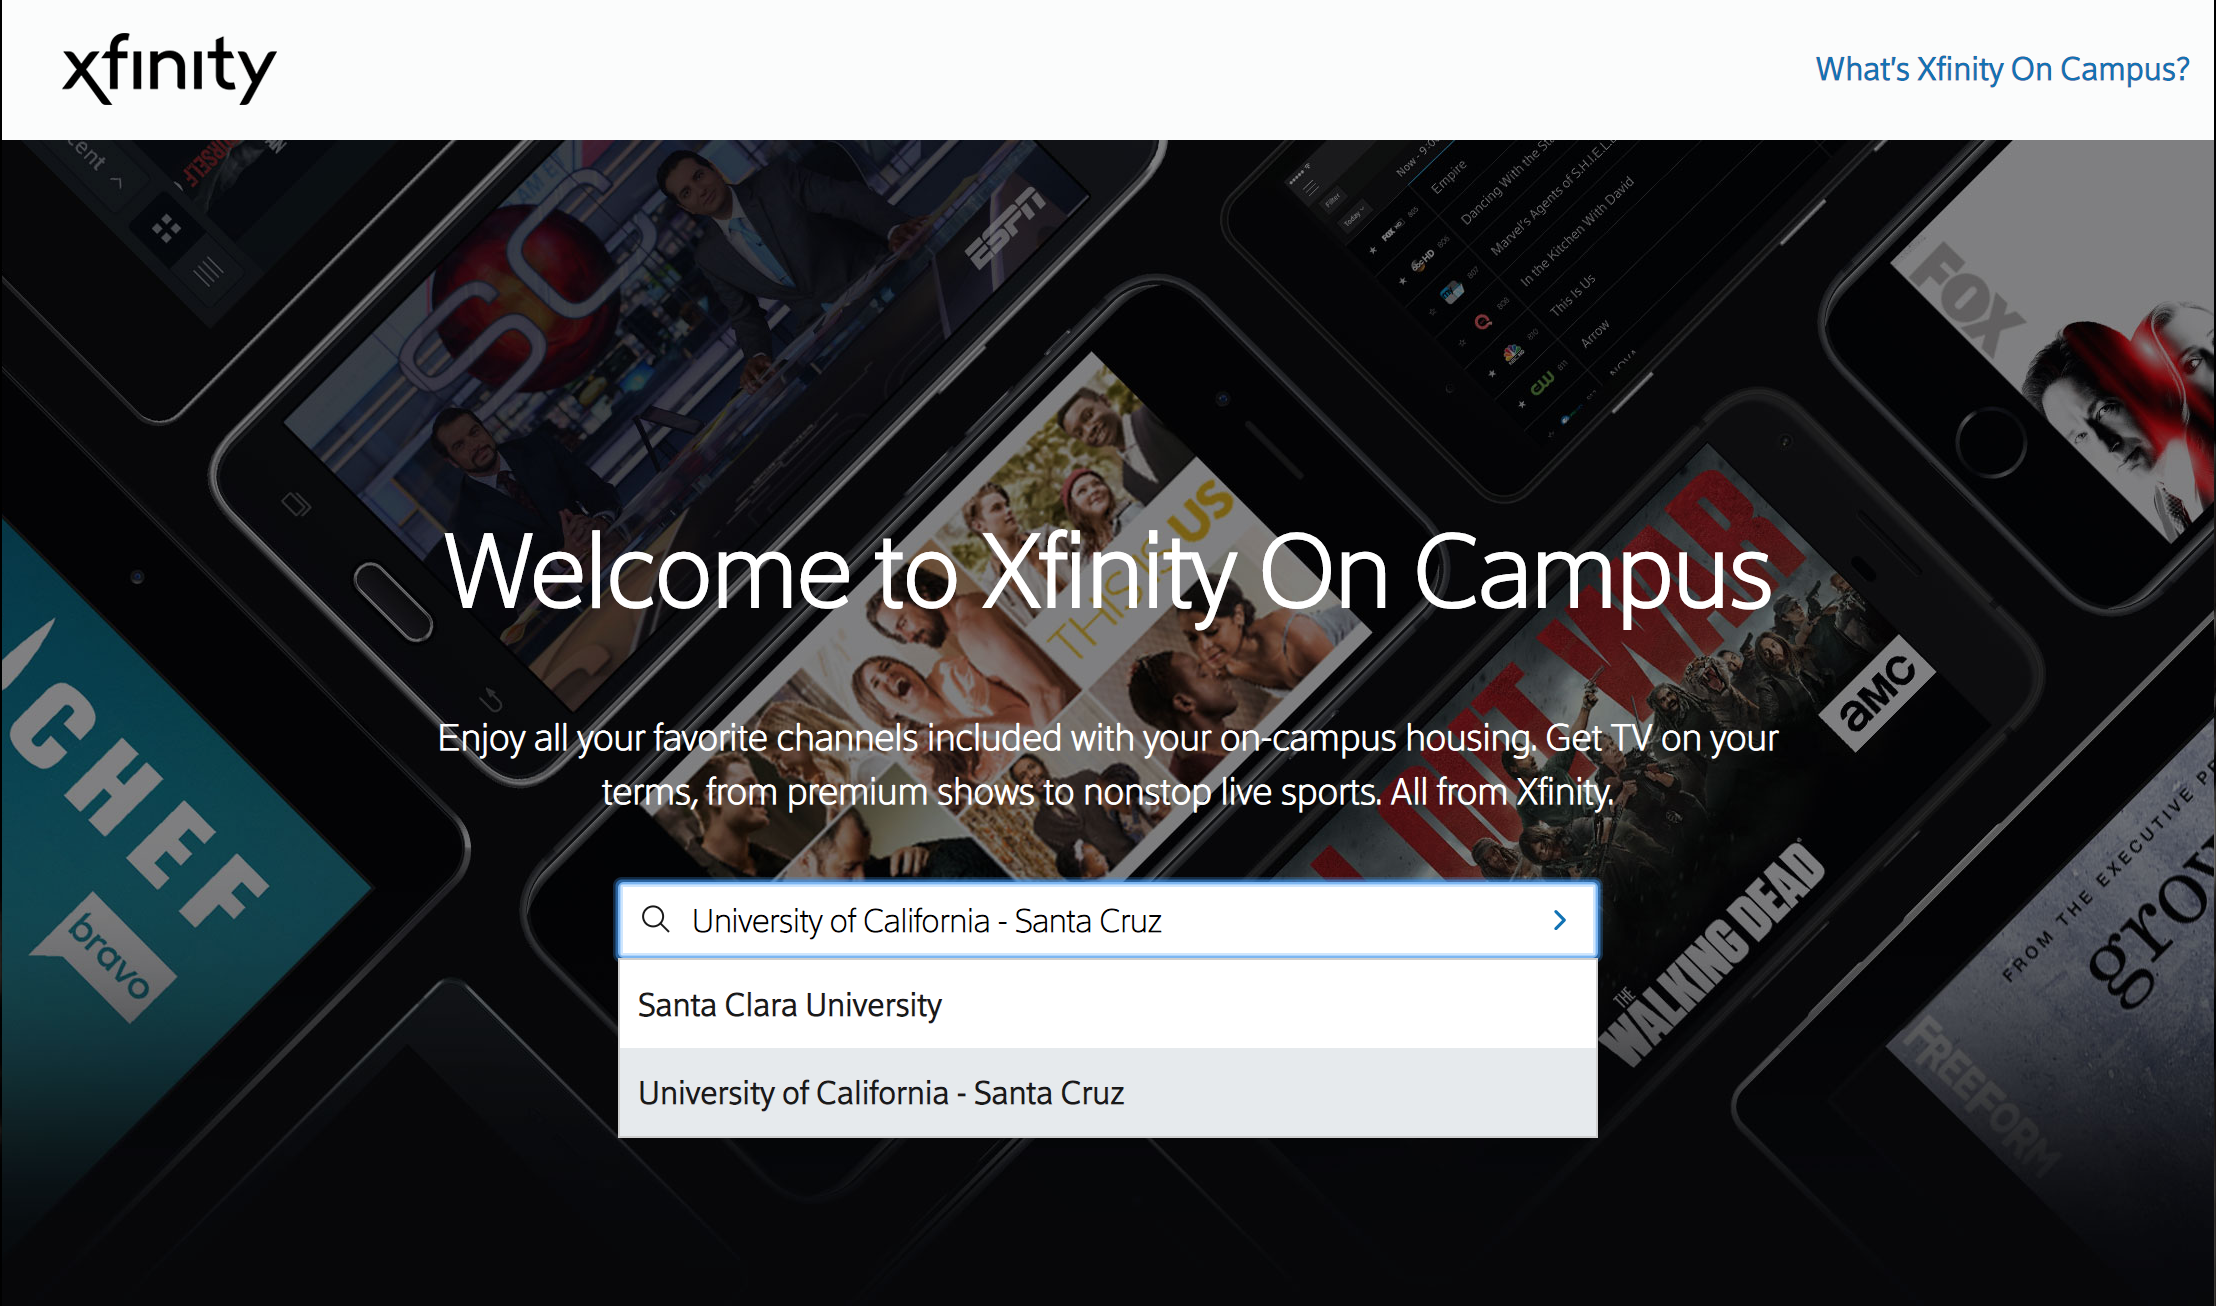
\includegraphics[width=\linewidth, height=\textheight, keepaspectratio]{welcome.png}
\begin{itemize}
  \item Enter your cruz credentials, afterwards youll be directed to a new URL
  https://www.xfinity.com/stream/.  Note: you may get taken to an intermediary
  information release page from 
  https://login.ucsc.edu/  You may proceed accept and proceed.

  \item Once you are on logged in to the stream site, the two fields most
  pertinent to watching television are \textbf{Channels} (peach) and 
  \textbf{Watch Now}
  (red).
\end{itemize}

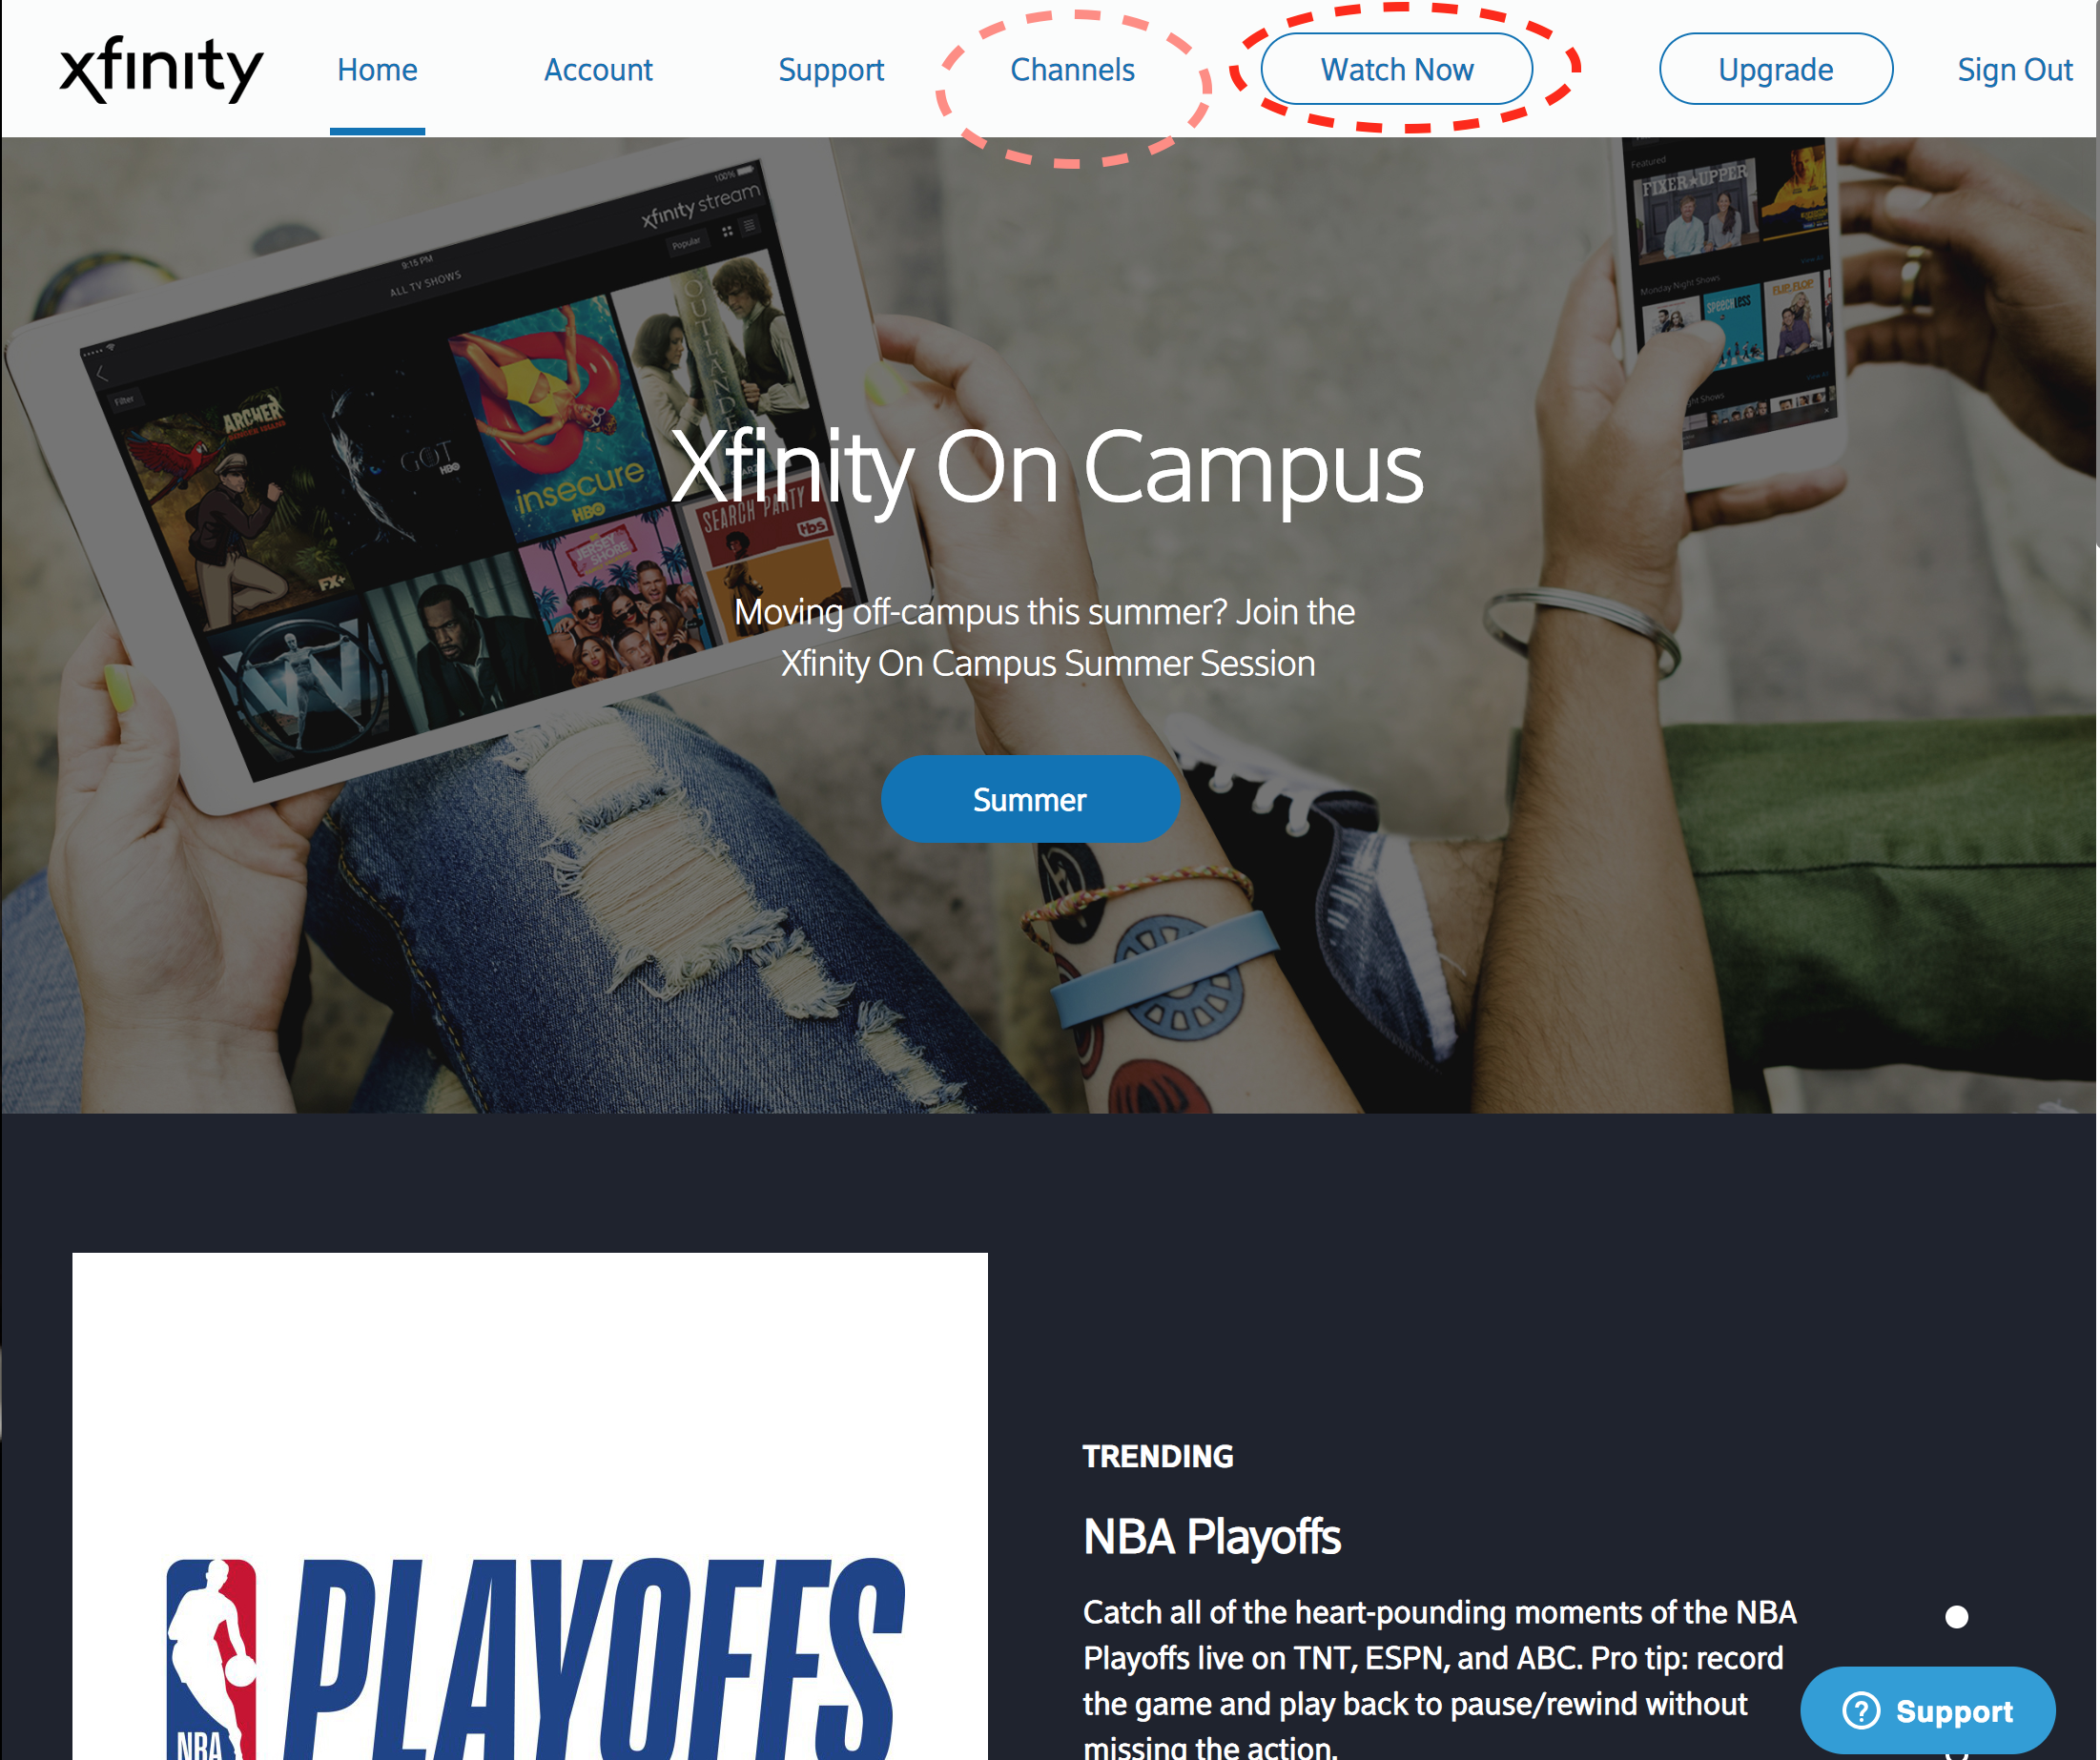
\includegraphics[width=\linewidth, keepaspectratio]{home.png}
\section*{
  Channels 
}

Channels is a useful interface that shows the current channel lineup.  This 
is useful for your television if you are not using a computer to watch and
would like to know the channel guide.  An important distinction to make is 
that if you are using a coaxial connection for television, you may not
receive all the channels listed in the channel section.  If you would like to
view the subset of channels not going through the coax connection, you may
use a computer and stream it to your TV either via connecting through a 
cable (hdmi, vga + audio etc) or through a streaming device such as a Chromecast.

When a desired channel or show is found, upon selecting \textbf{Watch Now} you
will be directed to the same URL as if you had selected \textbf{Watch Now} on
the Xfinity stream page.

\section*{
  Watch Now
}

Watch Now allows you stream from available programs, watch live TV, and record television programs.  To reiterate, this page will not work in a private 
browsing window and you must have flash enabled.  

\begin{itemize}
  \item Streaming is as simple as browsing through available on demand 
  programs and selecting the one you want to watch.
  \item Live TV can be found by selecting the \textbf{Live TV} drop down 
  header menu item and selecting \textbf{All Channels}.  Once you click
  on a channel, you may either watch, record, or view more information
  about the program.
\end{itemize}
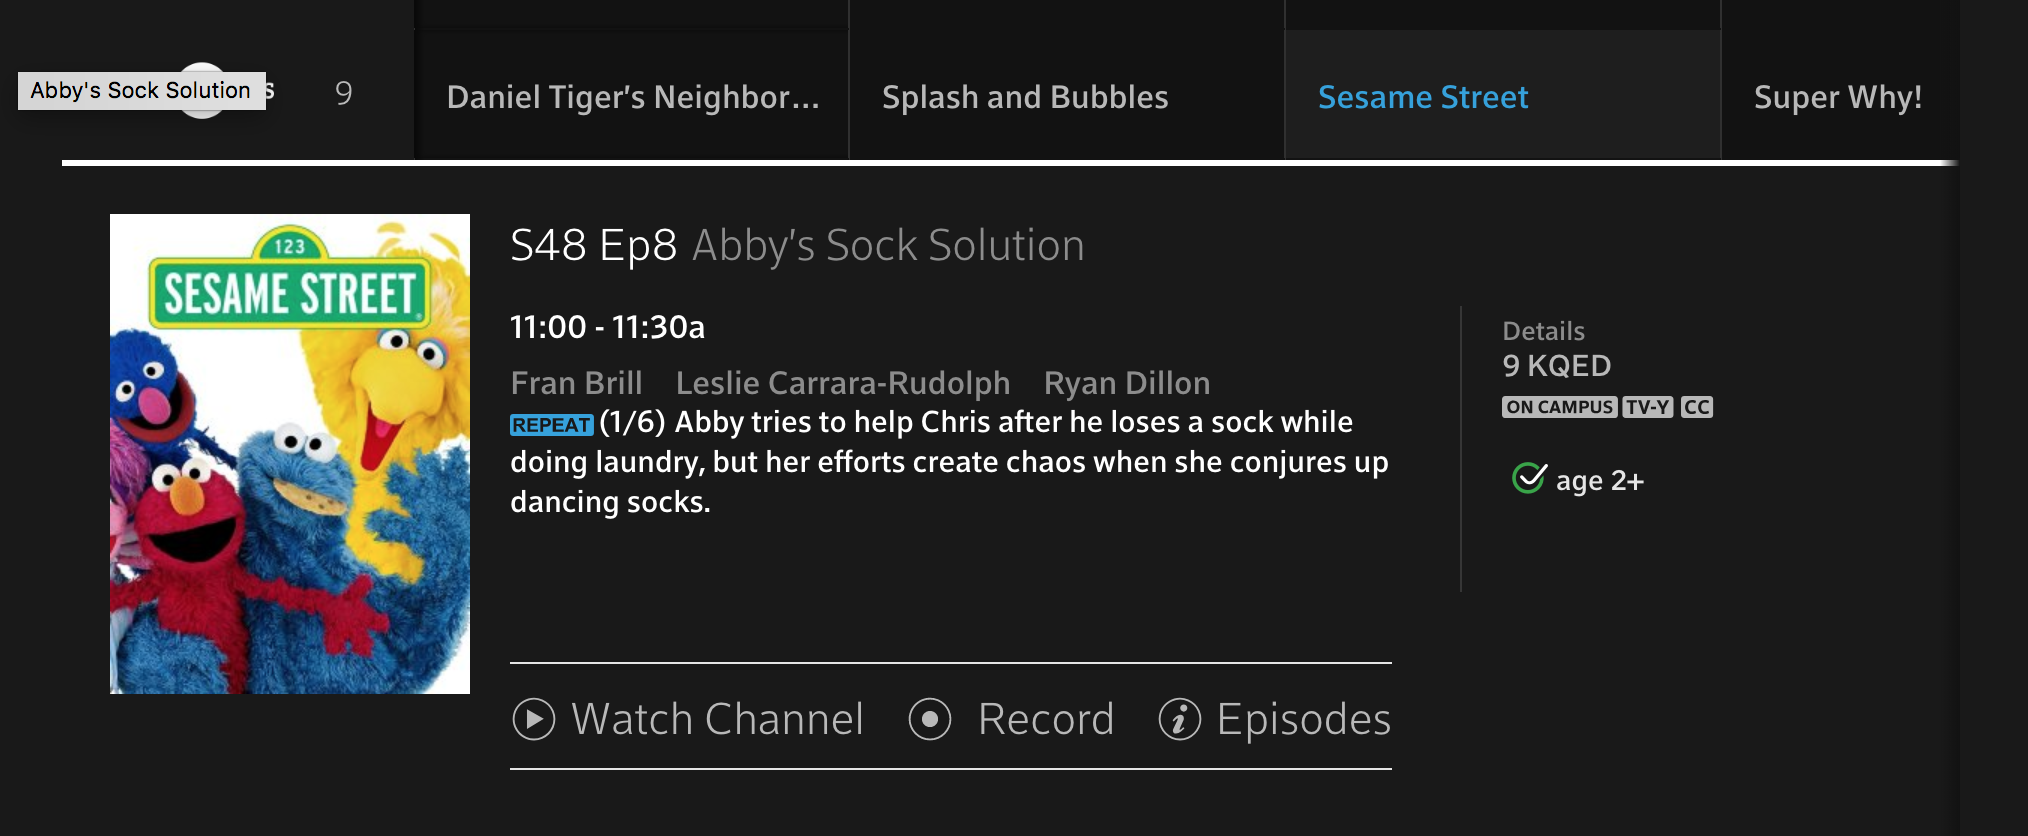
\includegraphics[width=\linewidth, keepaspectratio]{seas.png}
\begin{itemize}
  \item Recording shows is possible with the record option.  Once selected
  you may choose to record one episode or the entire series.  Recordings 
  can be viewed/managed by selecting the \textbf{Saved} drop down header
  menu item and selecting \textbf{Recordings}
\end{itemize}
\end{document}

